%!TEX root = ../thesis.tex
\chapter{Extraction of 3D Anatomical Structure} % (fold)
\label{cha:extraction_of_3d_anatomical_structure}

% If you like chapter abstracts ...
\dblspace
\begin{quote}{\em %!TEX root = ../thesis.tex

explicitly state what is my contribution. 
}\end{quote}

\section{Aims} % (fold)
\label{sec:aims}
  Having obtained a coherent histological volume in a region around an epicardial vessel, the challenge remains to extract an accurate, anatomically based model of tissue microstructure from the volume, firstly as an anatomical reference, but also to perform realistic simulations investigating the role of microstructure in electrophysiological wave propagation, and quantifying the functional consequences of incorporating microstructure into models. In this chapter, we extract volumetric image gradients using what is known as the structure tensor, in the hope that these gradients will correlate closely with the local myocardial fibre direction. We find that in this case, even extremely small displacements of the slices relative to each other is enough to drown the gradient signal from the fibre direction.
% section aims (end)

\section{Methods} % (fold)
\label{sec:methods}
  We can construct a matrix $S_0$ from the Cartesian product of the gradient of an image $I$. For illustrative purposes, let us consider a 2-dimensional image $I(x,y)$, so that
  
  \begin{align}
    S_0 &= \nabla I^T \, \nabla I \\
        &= \begin{pmatrix}
      I_x \\
      I_y
    \end{pmatrix} \begin{pmatrix}
      I_x && I_y
    \end{pmatrix} \\
        &= \begin{pmatrix}
          I_x^2 && I_xI_y \\
          I_xI_y && I_y^2
        \end{pmatrix}.
  \end{align}
  
  Because of the associativity of matrix multiplication, we can see that a multiplication of a vector $v$ with any matrix constructed from the Cartesian product of a vector $u$ will simply result in a vector parallel to $u$, with magnitude equal to the dot product of $v$ and $u$ multiplied by the magnitude of $u$. In our case,
  
  \begin{align}
    S_0 \mathbf{v} &= (\nabla I^T \, \nabla I) \mathbf{v} \\
                   &= (\nabla I \cdot \mathbf{v}) \nabla I^T.
  \end{align}
  
  From this it is clear that $S_0$ is a tensor with two eigenvectors, parallel with and perpendicular to $\nabla I$, with eigenvalues of $|\nabla I|^2$ and 0, respectively.
  
  The structure tensor $S_w$ is a matrix derived from this Cartesian product of the gradient of an image, which gives a measure of the magnitude and coherence of changes in intensity across a small image region. It is defined as the weighted mean of $S_0$ within a surrounding window $w$ of a given point in $I$. Equivalently, it is the convolution of $S_0$ with the windowing function.
  
  If the gradients are all coherently aligned well within a window, the largest eigenvector of the resulting $S_w$ will be much greater than the other eigenvectors, and in 3-D, the tensor will take a long, thin shape. Clearly, $S_0$ is itself perfectly coherent. Gradients may also be distributed throughout a subspace of the entire space; in 3-D, gradients varying evenly within a 2-D plane will result in a flat, disc-shaped tensor, with one small eigenvalue associated with a vector perpendicular to that plane. If gradients are more isotropic, then all eigenvalues will be of a similar magnitude, giving a spherical tensor, and a zero tensor can only obtained if the gradient is zero throughout the windowing region.
  
  In a perfectly registered histological volume, and at the scale of individual myocardial cells, the smallest intensity gradients will be found parallel to the fibre direction, and the largest in the plane perpendicular to them. The structure tensors should therefore appear disc-shaped, with their short axis aligned with the muscle fibres. At the larger scale of myocardial sheets, we would expect javelin-shaped tensors with one eigenvalue much larger than the other two, oriented perpendicularly to the sheet plane. In this case, and depending on scale and smoothing, we might expect that the smallest eigenvalue would be oriented in the predominant fibre direction.
  
  We apply the structure tensor to the regionally registered block from Section~\ref{sub:regional_diffusion}. It is important to have the same sampling rate within the plane of the slices as between them, so that artificial anisotropy is not introduced. A volume is therefore constructed from slice images that are downsampled and Gaussian smoothed so as to have the same spatial resolution of 10$\mu$m as the slicing. A Gaussian windowing kernel is applied to the structure tensor volume, with $\sigma$ equal to the pixel spacing.
% section methods (end)

\section{Results} % (fold)
\label{sec:results}
  \begin{figure}[htbp]
    \centering
    \subfigure[][im2]{\includegraphics[width=0.24\textwidth]{Ch7/Figs/2D/01_im2.png}}
    \subfigure[][threshold image]{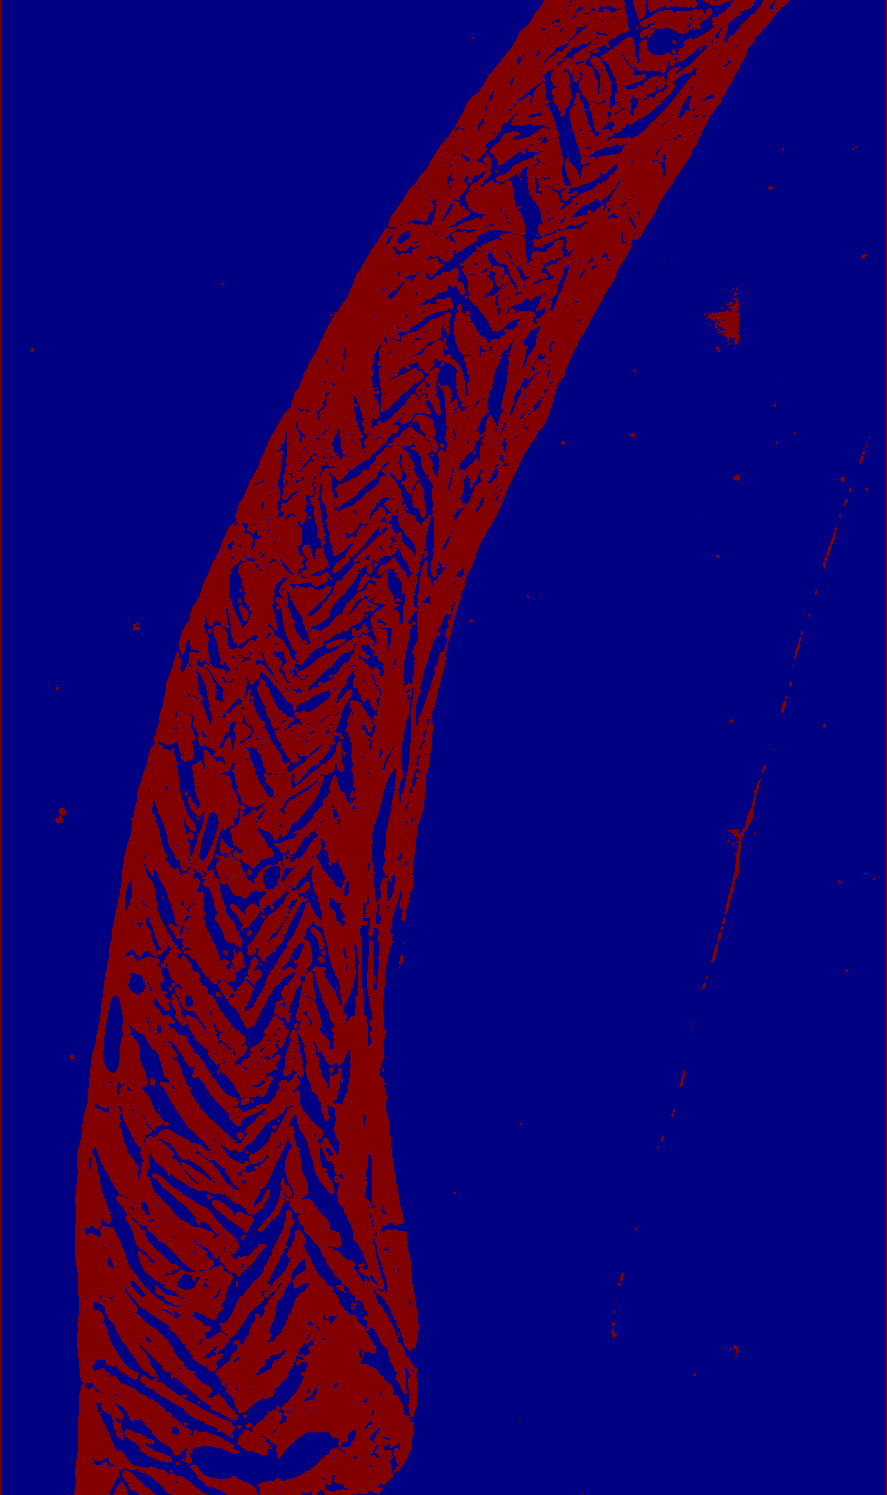
\includegraphics[width=0.24\textwidth]{Ch7/Figs/2D/02_threshold_image.png}}
    \subfigure[][closed and opened threshold image]{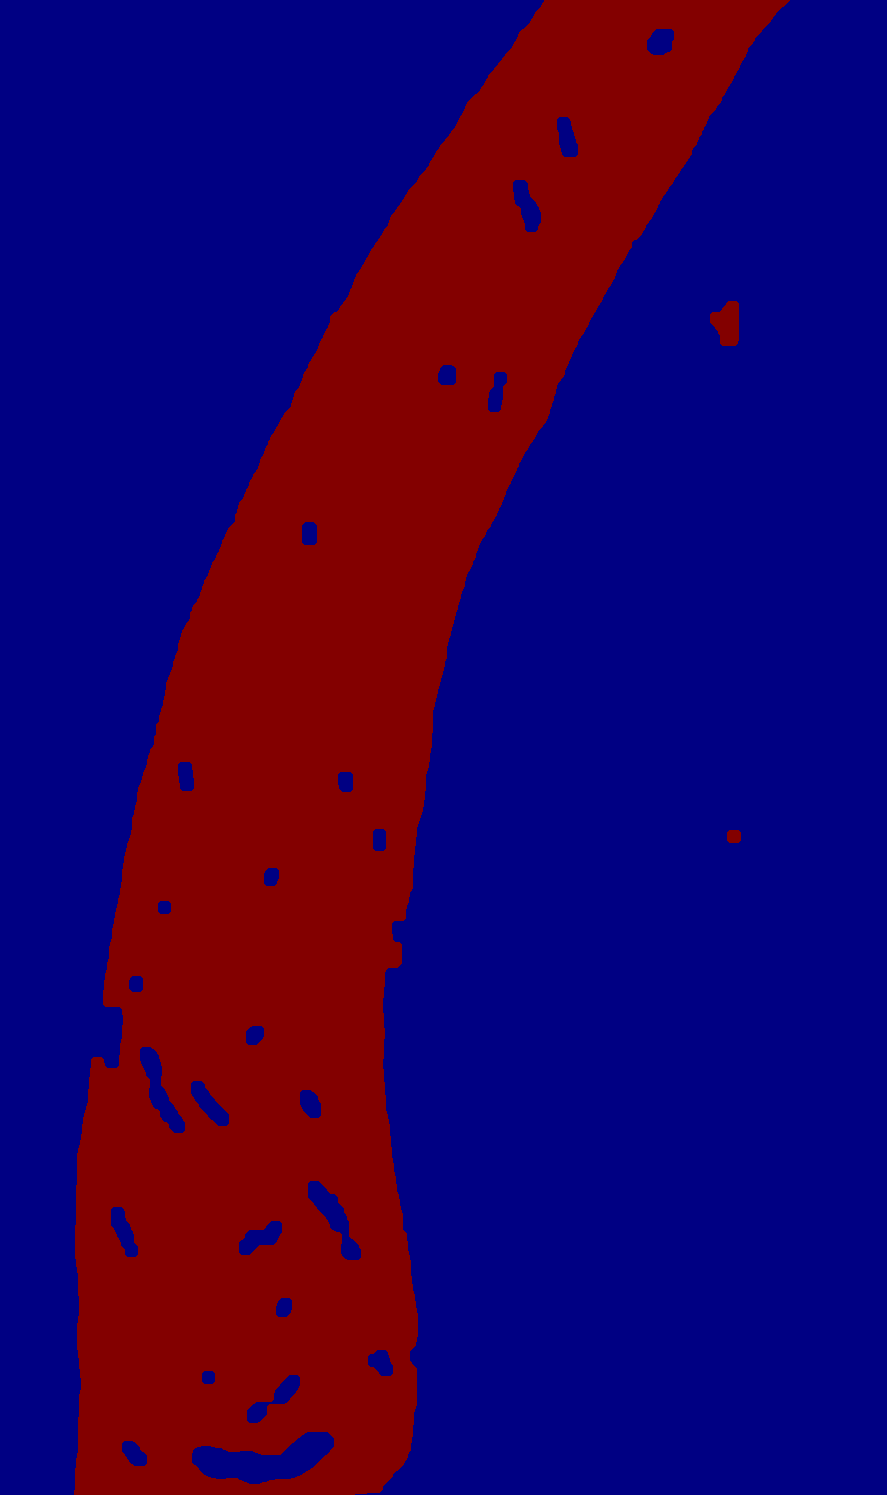
\includegraphics[width=0.24\textwidth]{Ch7/Figs/2D/03_closed_and_opened_threshold_image.png}}
    \subfigure[][non tissue label image]{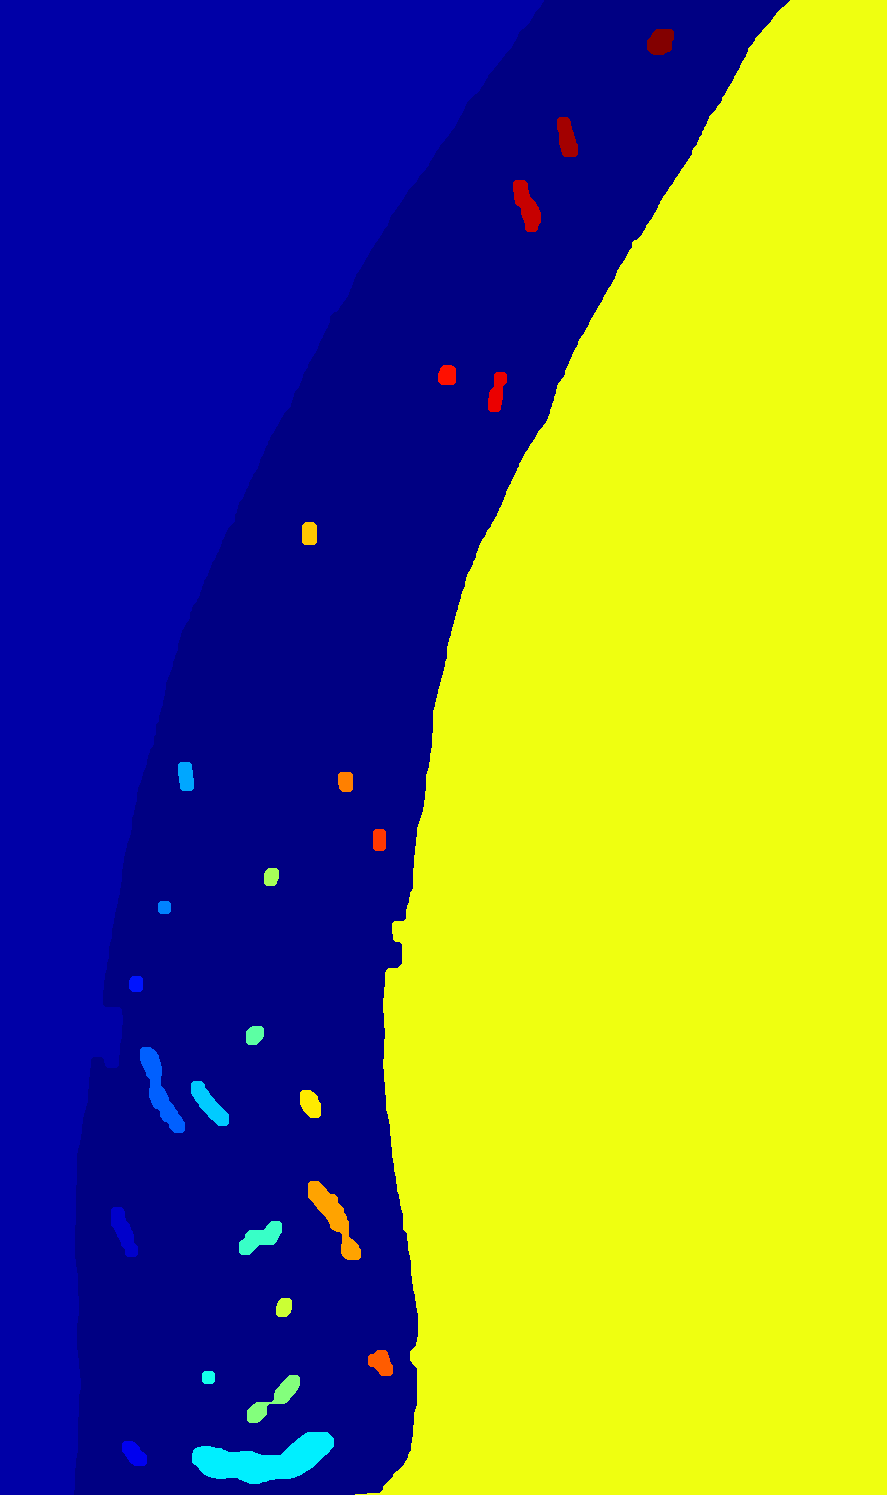
\includegraphics[width=0.24\textwidth]{Ch7/Figs/2D/06_non_tissue_label_image.png}}
    \caption{}
    \label{fig:2D_structure_tensor}
  \end{figure}
  
  \begin{figure}[htbp]
    \centering
    \subfigure[][clefts]{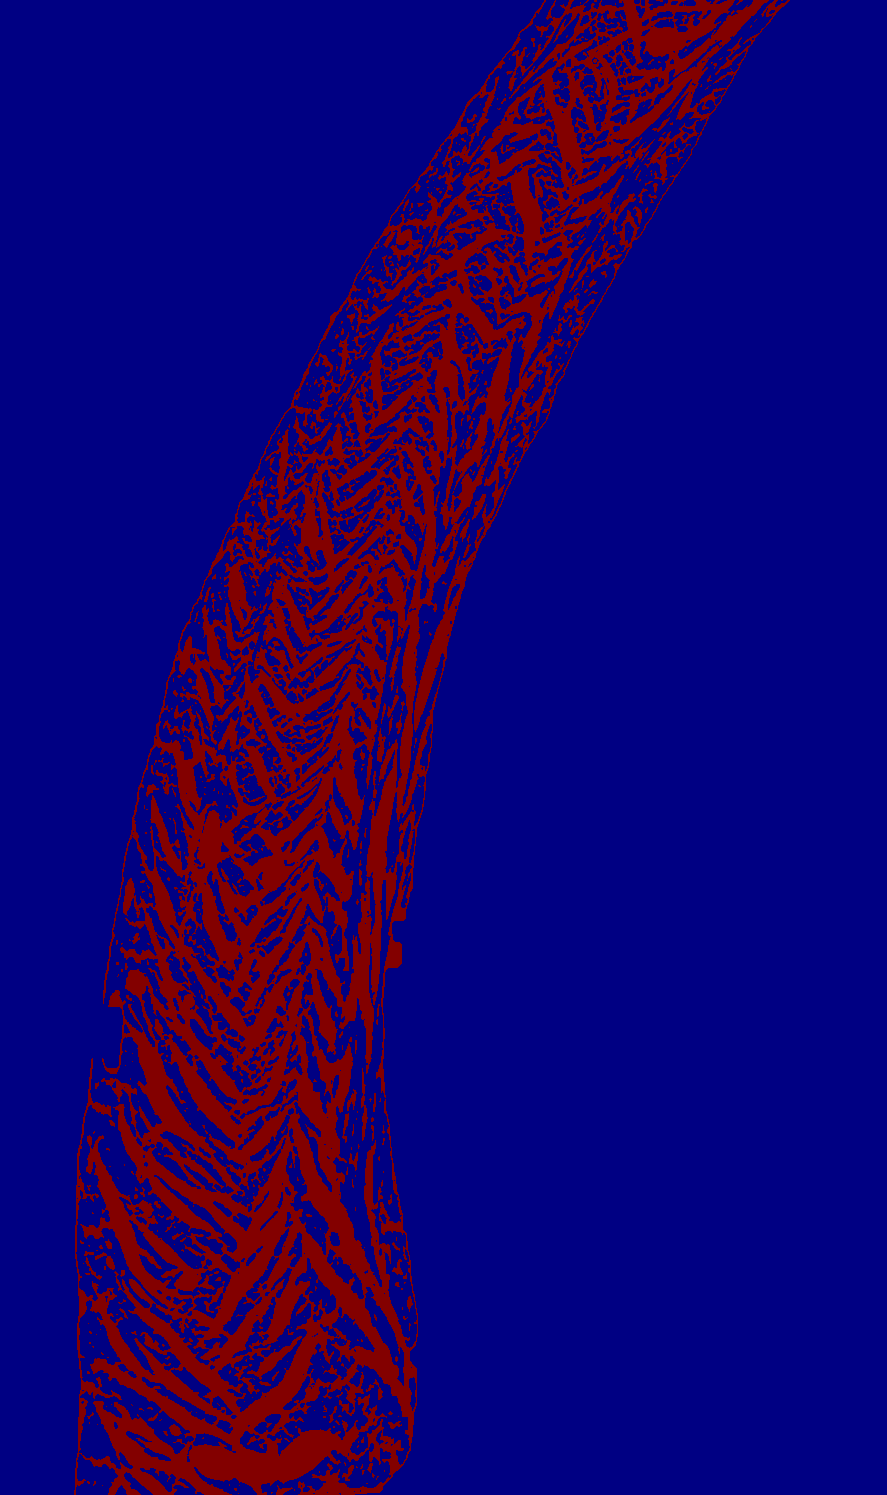
\includegraphics[width=0.24\textwidth]{Ch7/Figs/2D/10_clefts.png}}
    \subfigure[][clefts2]{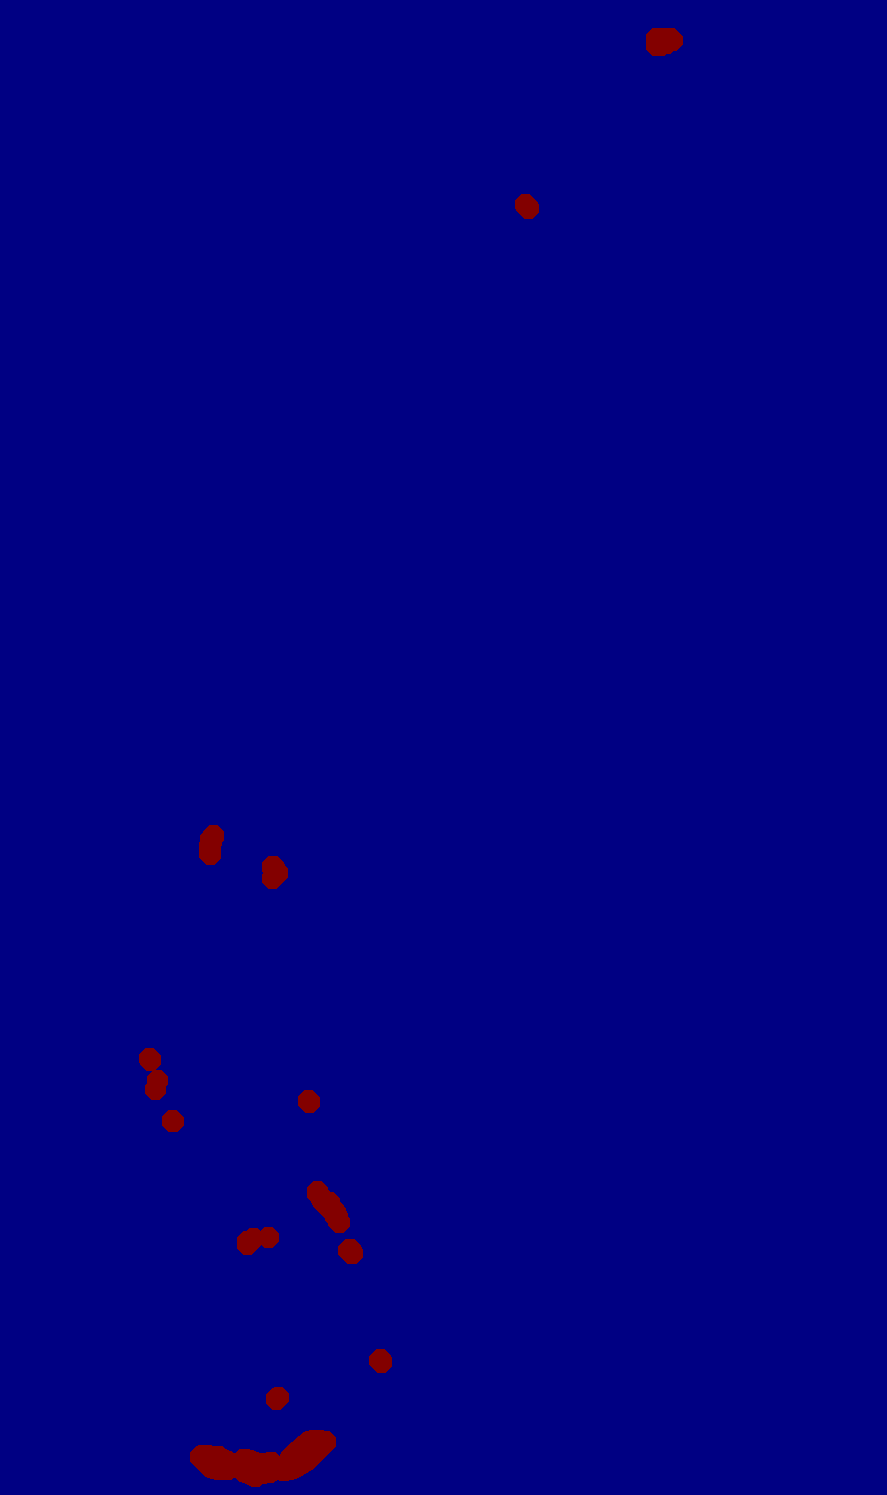
\includegraphics[width=0.24\textwidth]{Ch7/Figs/2D/11_clefts2.png}}
    \subfigure[][opened clefts]{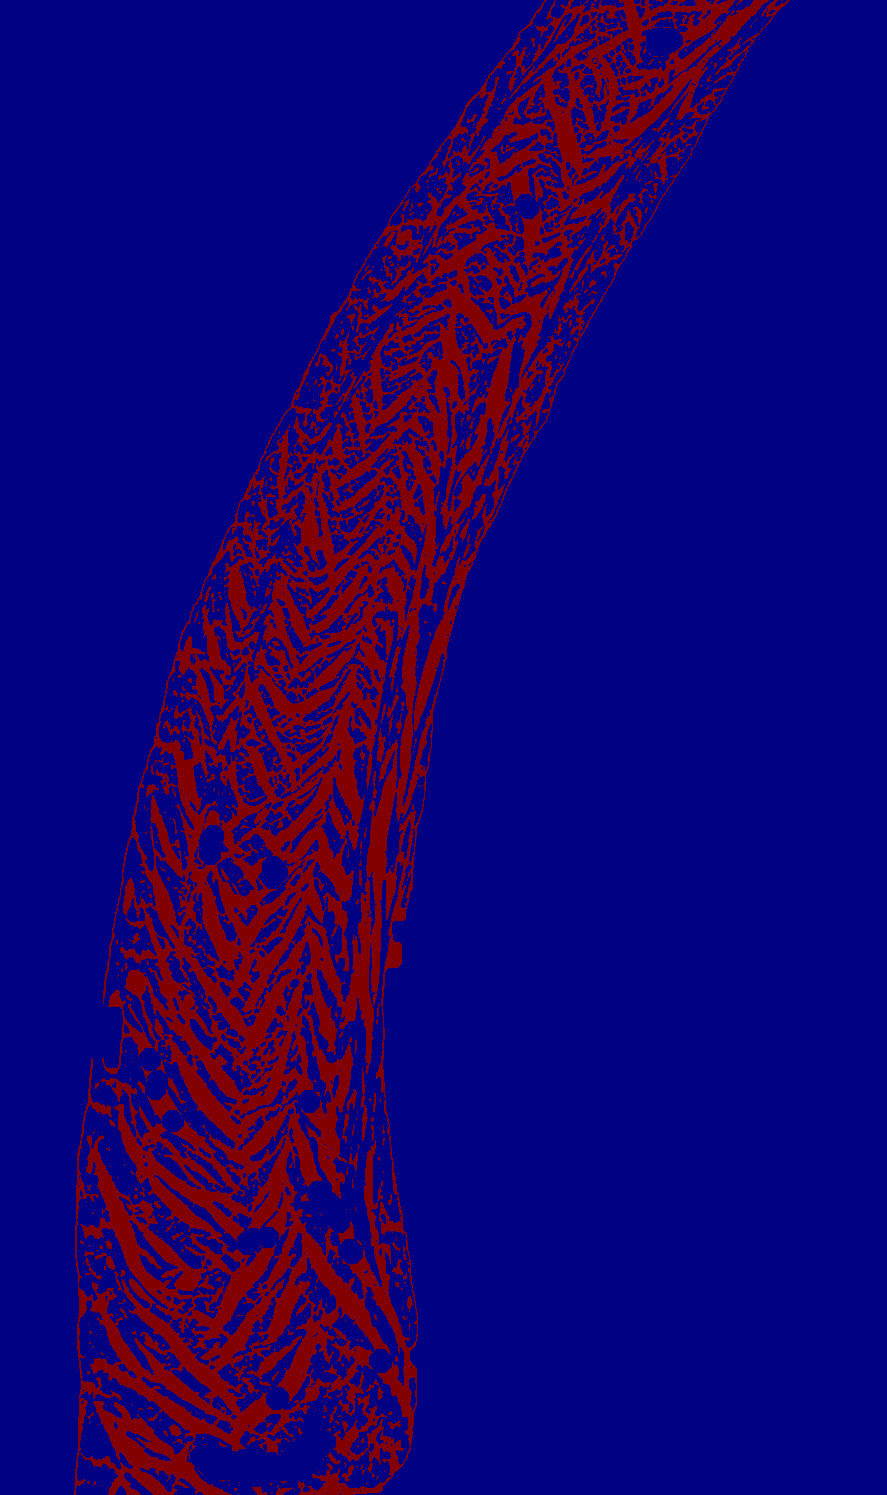
\includegraphics[width=0.24\textwidth]{Ch7/Figs/2D/12_opened_clefts.png}}
    \caption{Cleft extraction figure}
    \label{fig:2D_cleft_extraction}
  \end{figure}
  
  \begin{figure}[htbp]
    \centering
    \subfigure[][angles]{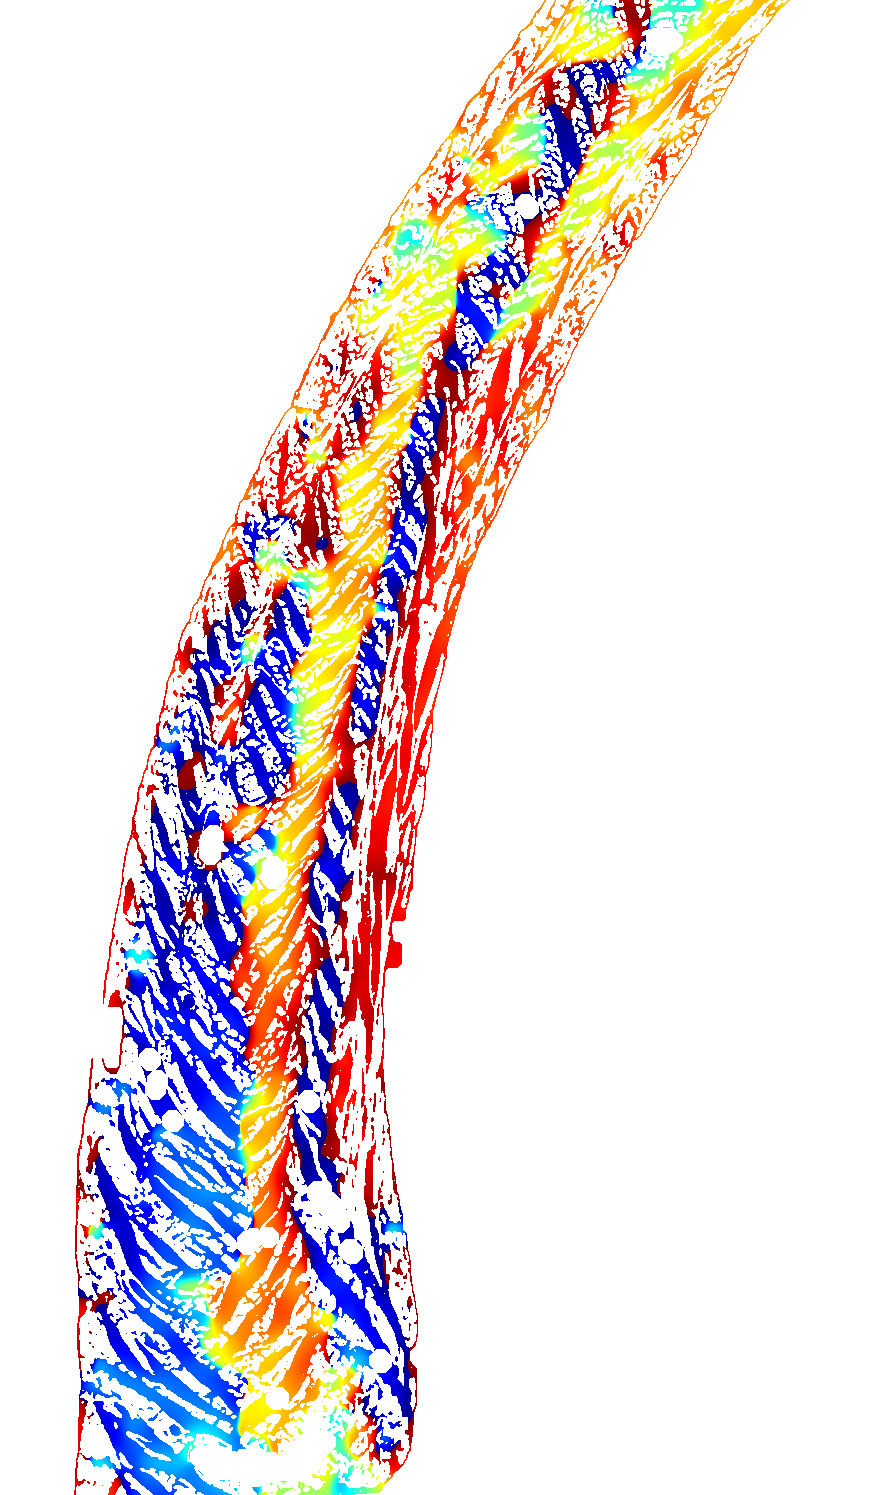
\includegraphics[width=0.24\textwidth]{Ch7/Figs/2D/13_angles.png}}
    \subfigure[][e]{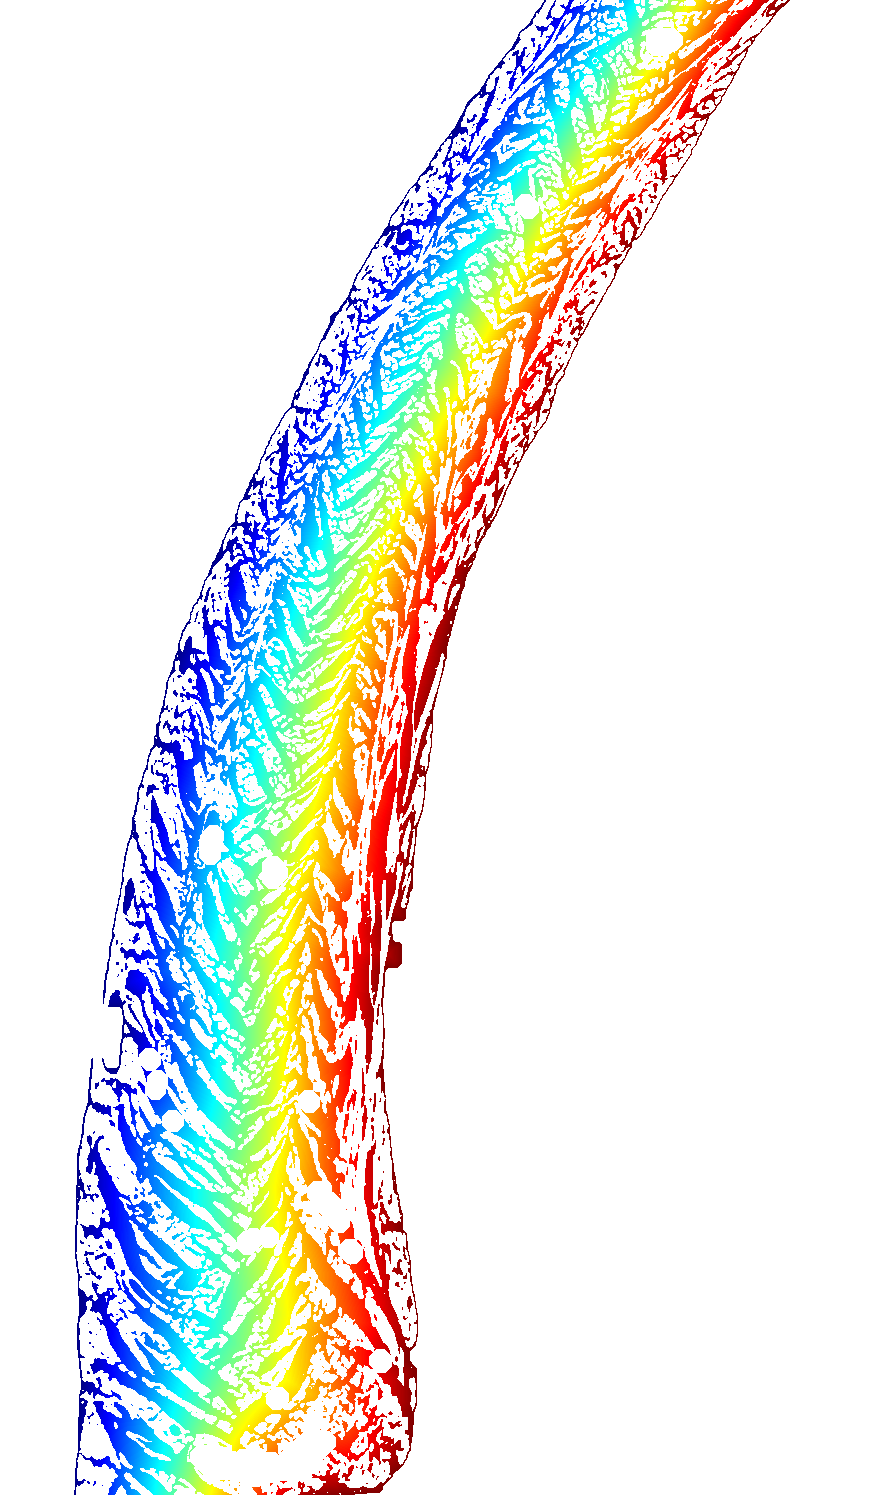
\includegraphics[width=0.24\textwidth]{Ch7/Figs/2D/14_e.png}}
    \caption{Angles and e figure}
    \label{fig:2D_angles}
  \end{figure}
  
  
  
  \begin{sidewaysfigure}[htbp]
    \centering
    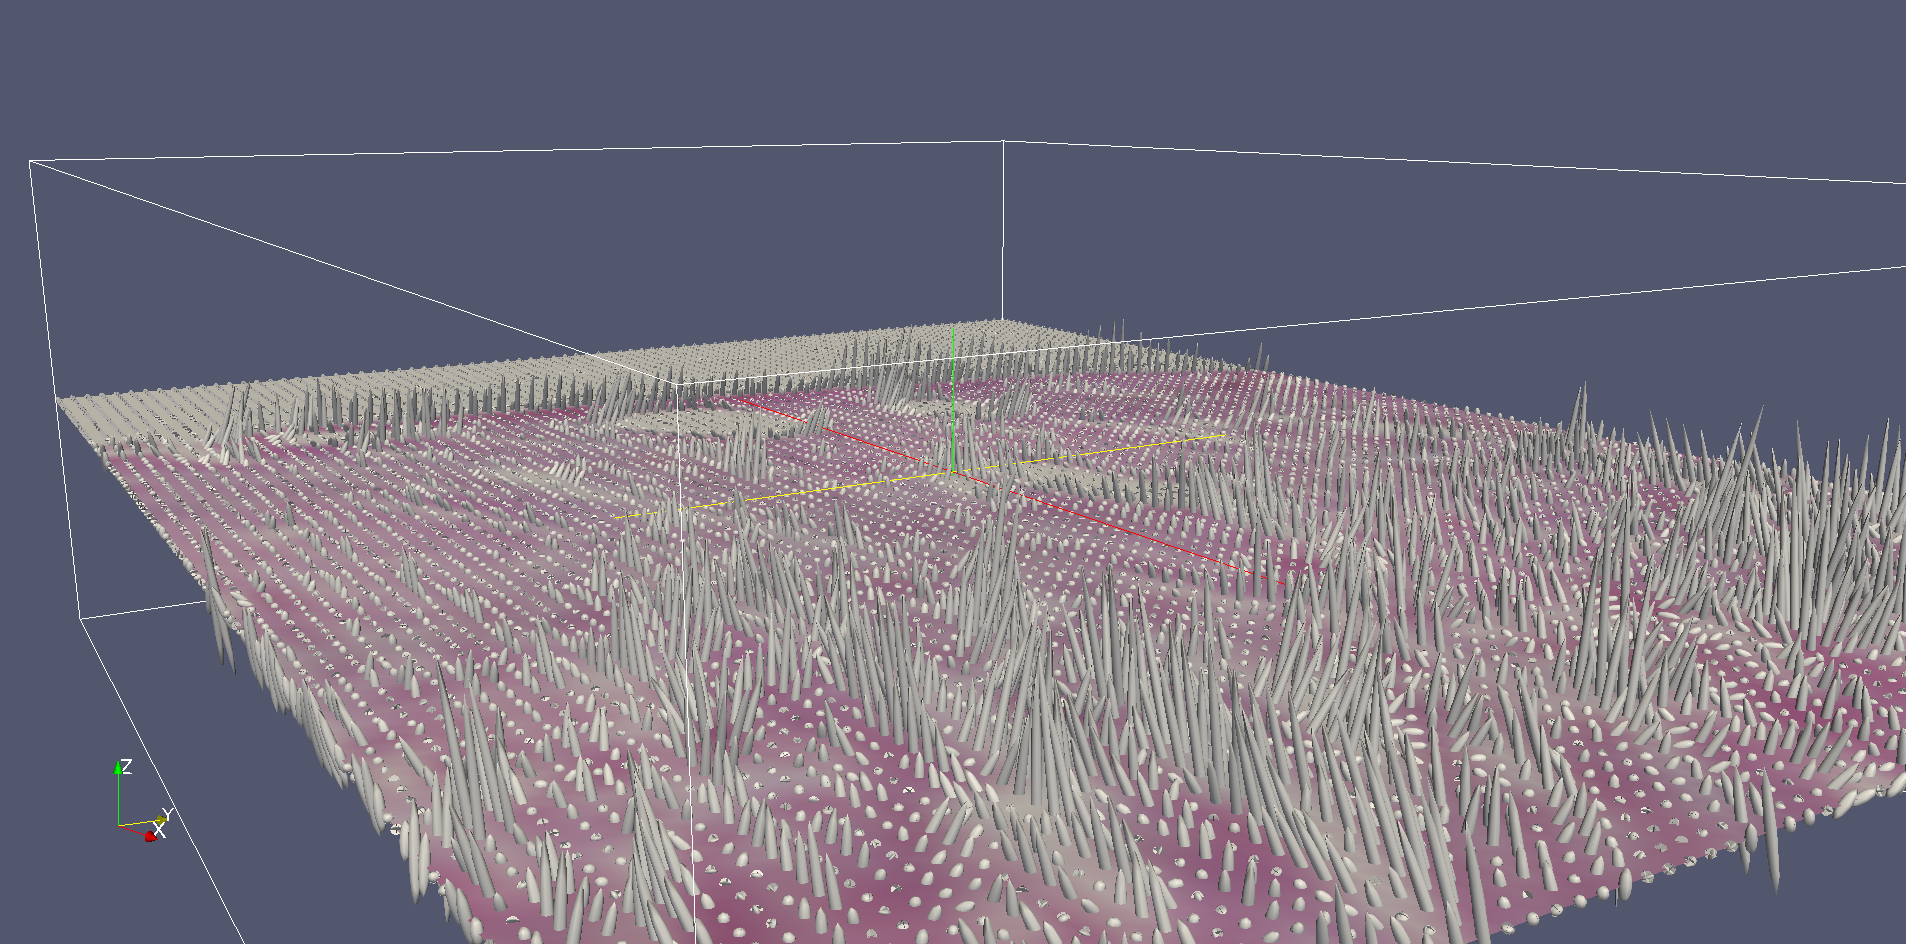
\includegraphics[width=\textwidth]{Ch7/Figs/structure_tensor_glyphs}
    \caption{A central slice through the epicardial vessel region from Section~\ref{sub:regional_diffusion}, overlayed with spheroid glyphs, scaled and oriented by the structure tensor of the pixel intensities.}
    \label{fig:structure_tensor_glyphs}
  \end{sidewaysfigure}
  
  \begin{figure}[htbp]
    \centering
    \subfigure[][x]{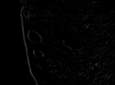
\includegraphics[width=0.45\textwidth]{Ch7/Figs/x_eigencomponent.png}}
    \subfigure[][y]{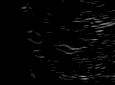
\includegraphics[width=0.45\textwidth]{Ch7/Figs/y_eigencomponent.png}}
    \subfigure[][z]{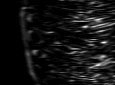
\includegraphics[width=0.45\textwidth]{Ch7/Figs/z_eigencomponent.png}}
    \subfigure[][combined]{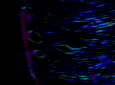
\includegraphics[width=0.45\textwidth]{Ch7/Figs/rgb_eigencomponents.png}}
    \caption{\textbf{(a)}, \textbf{(b)} and \textbf{(c)} map the absolute magnitudes of the x-, y- and z- components of the largest eigenvector of the structure tensor, of the same central slice from Figure~\ref{fig:structure_tensor_glyphs}. The volumewise maximums for the x-, y-, and z- components were 15.8, 14.6 and 68.7, respectively; the intensities have thus been scaled from 0 (black) to 68.7 (white). \textbf{(d)} combines the intensities in an RGB image, with red x, green y and blue z.}
    \label{fig:eigencomponents}
  \end{figure}
  
  Figure~\ref{fig:structure_tensor_glyphs} illustrates the form of the structure tensor across the central histological slice of the epicardial block. A regular grid of spheroid glyphs are plotted at each pixel of the slice, with principal axes aligned and proportional to the eigenvectors and eigenvalues of the structure tensor. It is evident that the largest tensors are not, as expected, disc-like, but in fact javelin-like, as one eigenvalue greatly exceeds the other two. It is also evident that larger tensors are oriented predominantly in the z-direction perpendicular to the plane. Figure~\ref{fig:eigencomponents} echoes this finding, showing grayscale images of the magnitudes of the three components of the largest eigenvector. By far the brightest image is that of the z-component. This dominance is also expressed in the largely blue appearance of Figure~\ref{fig:eigencomponents}(d), with only small tinges of red and green.
% section results (end)

\section{Discussion} % (fold)
  The dominance of intensity gradient in the z-direction is a result of slices being very slightly out of alignment with each other, by the distance of the width of a cell or greater. Unfortunately, the misalignment often leads to a `zig-zagging' of intensities perpendicular to the slices and at the frequency of the slicing, which manifests as an inflated z-gradient. An attempt to extract fibre direction and incorporate this information into a model for simulation would sadly be fruitless in this context.
  
\label{sec:discussion}
  
% section discussion (end)

% chapter extraction_of_3d_anatomical_structure (end)
